\chapter{Manifold Theory}\label{ch:manifold-theory}
\begin{chout}
	The following chapter serves as an introduction to manifold theory which,
	through specification, will arrive us at the notion of a Riemann surface.
	The definitions are similar to those found in Lee\sidenotemark.
\end{chout}
\sidenotetext[][5\baselineskip]{\footnotesize\cite{lee}}

\section{Topological manifolds}
With an understanding of the direction in which our consideration is headed, we
introduce the following concepts in their complex version. There are times
however, when further intuition may be gained by consideration of the real
analogues of the definitions, and examples will be given when this is the case.
We start with a basic topological idea.

\begin{definition}[Hausdorff]
	A topological space $ X $ is \defined{Hausdorff} if for all distinct points $
		u,v \in X $ there exist open sets $ U \ni u $, $ V \ni v $ such that $ U \cap V
		= \varnothing $.
\end{definition}

\begin{marginfigure}
	\centering
	\includegraphics{hausdorff/figure}
	\caption{A Hausdorff space.}
\end{marginfigure}

\begin{example}\label{ex:complex-plane-discrete}
	Let $ \mathbb{C} $ have the discrete topology, that is, the topology with the
	basis of singleton sets in $ \mathbb{C} $. It is trivial that this space is
	Hausdorff; two distinct points $ z, \omega \in \mathbb{C} $ can be separated by
	their respective singletons, $ \left\{ z \right\} \cap \left\{ \omega \right\}
		= \varnothing $.
\end{example}

\begin{definition}[Locally Euclidean]
	Let $ X $ be a topological space. We say that $ X $ is \defined{locally
		Euclidean} of dimension $ n $, if for each $ x \in X $ there exists an open
	neighbourhood $ U_x $ of $ x $ homeomorphic, via homeomorphism $ \phi_x $, to an
	open subset $ \tilde{U}_{x}\subseteq \mathbb{C}^{n} $.
\end{definition}

\begin{marginfigure}[-3\baselineskip]
	\centering
	\includegraphics{s2-manifold/figure}
	\caption{$ S^2 $ is (real) locally Euclidean of dimension $ 2 $.}
\end{marginfigure}

\begin{remark}
	It is important to mention that reference to dimension will be implicit reference
	to \textit{complex} dimension, unless otherwise specified.
\end{remark}

The homeomorphisms, $ \phi_x $, are called \defined{coordinate functions}
(sometimes coordinates) at $ x $, motivated by the fact that they provide a
local Euclidean coordinate system on the space. Together with the domains on
which they are defined, coordinate functions are called \defined{charts},
denoted by $ (U_x, \phi_x) $. Any collection of chart domains which provides an
open cover of the space is called an \defined{atlas}, $ \{ U, \phi \} $.

\begin{example}[Complex plane with two
		origins]\label{ex:complex-plane-2-origins}
	Consider the space $ L $, constructed by taking two copies of $ \mathbb{C} $ and
	identifying all identical points apart from the origins. With greater formality,
	let
	\begin{gather*}
		L = \left( 0_a \times \mathbb{C} \sqcup 0_b \times \mathbb{C} \right)/{\sim}\\
		(0_a,z) \sim (0_b , z) \quad \forall z \in \mathbb{C}\setminus \left\{ 0 \right\}.
	\end{gather*}
	\begin{center}
		\begin{tikzpicture}
			\node (o) at (0,0){};
			\draw (-4,0) to (o);
			\draw (o) to (4,0) node[right]{$ \mathbb{C} $};
			\fill ($ (o) + (0,0.1) $) circle (0.05) node[above]{$ 0_a $};
			\fill ($ (o) - (0,0.1) $) circle (0.05) node[below]{$ 0_b $};
		\end{tikzpicture}
	\end{center}
	Describing the quotient topology on this space is straightforward; we can form a
	basis as follows. Firstly, we take the open sets of $ \mathbb{C}^{*} :=
		\mathbb{C}\setminus \left\{ 0 \right\} $, and join this collection with sets $
		(U \setminus \left\{ 0\right\}) \cup \left\{ 0_i \right\} $, for open $ U \subseteq
		\mathbb{C} $ containing $ 0 $.

	Since $ \mathbb{C}^{*} \subseteq \mathbb{C} $, we need only check if the two
	origin points $ 0_a $ and $ 0_b $ are locally Euclidean. The open neighbourhoods $
		\mathbb{C}_{i}:=\mathbb{C}^{*}\cup \left\{ 0_i \right\} $ of $ 0_i $ are both
	homeomorphic to $ \mathbb{C}$ via
	\begin{align*}
		\phi_i: \mathbb{C}_{i} \to \mathbb{C}: z \mapsto \begin{cases}
			                                                 z & z \in \mathbb{C}^{*} \\
			                                                 0 & z = 0_i
		                                                 \end{cases}
	\end{align*}
	and hence $ L $ is locally Euclidean of dimension $ 1 $.
\end{example}

Motivated in part by the existence of a few pathological counterexamples, the
definition of a topological manifold is often stated with the extra condition of
second-countability\sidenote{\footnotesize\cite[p. 36]{lee}}.

\begin{definition}[Second countability]
	A topological space $ X $ is called \defined{second countable} if it admits a
	countable basis for its topology.
\end{definition}

\begin{example}\label{ex:complex-cross}
	Let $ X = \left\{ (x,y) \in \mathbb{C}^{2}: xy=0 \right\} $. We aim to show that
	this set has a countable basis for the subset topology from $ \mathbb{C}^{2} $.
	Firstly, we note that $ \mathbb{R} $ admits a basis
	\begin{align*}
		\mathcal{B} = \left\{ (r,s) : r,s \in \mathbb{Q} \right\},
	\end{align*}
	i.e., the collection of open intervals in $ \mathbb{R} $ with rational
	endpoints. Further, $ \mathcal{B} $ has the same cardinality as $
		\mathbb{Q}^{2} = \mathbb{Q}\times \mathbb{Q} $ which is countable as the
	cartesian product of two countable sets (Figure~\ref{fig:Q-countable}). In
	particular, $ \mathbb{R} $ is second countable.

	$ \mathbb{R}^{4} $ is second countable when viewed as the fourth
	product of $ \mathbb{R} $ endowed with the product topology and since $
		\mathbb{R}^{4} \cong \mathbb{C}^{2} $, $ \mathbb{C}^{2} $ is also second
	countable. Finally, since second countability is hereditary, our claim is
	justified.
\end{example}

\begin{marginfigure}[-15\baselineskip]
	\centering
	\resizebox{\columnwidth}{!}{
		\includegraphics{Q-countable/figure}
	}
	\caption{$ \mathbb{Q} $ is countable.}
	\label{fig:Q-countable}
\end{marginfigure}

It is interesting to note that a restriction to topological spaces with
countable topologies is too heavy-handed. We would like to be able to consider
$ \mathbb{C} $ as a manifold, but even this space has uncountably many open
sets.

\begin{definition}[Topological manifold]
	An $ n $-dimensional \defined{topological manifold} is a second-countable,
	Hausdorff space, which is locally Euclidean of dimension $ n $.
\end{definition}

\begin{nonexample}
	Example~\ref{ex:complex-cross} is not locally Euclidean.

	Example~\ref{ex:complex-plane-2-origins} is not Hausdorff.

	Example~\ref{ex:complex-plane-discrete} is not second countable.
\end{nonexample}

\begin{example}\label{ex:C-top-manifold}
	Trivial examples of topological manifolds are $ \mathbb{C}^{n} $ with the
	standard topology, and subsets $ U \subseteq \mathbb{C}^{n} $ with the induced
	subset topology. The identity map over the whole space provides a suitable atlas
	in both cases.
\end{example}

Before examining further non-trivial examples in detail, we consider the
imposition of further structure on a manifold, as this leads the way to more
interesting results.

\section{Complex analytic manifolds}
Further restrictions on manifolds are imposed via the charts which define them.

\begin{definition}[Compatible charts]
	The charts $ (U_x, \phi_x) $ and $ (U_y, \phi_y) $ on a topological space $ X $
	are said to be \defined{compatible} if
	\begin{align*}
		\phi _{x,y}:= \phi_x \circ \phi_y ^{-1}: \phi_y(U_x \cap U_y) \to \phi_x(U_x
		\cap U_y)
	\end{align*}
	is holomorphic. Charts are \defined{vacuously compatible} if $ U_{x}\cap
		U_{y}\neq\varnothing $.
\end{definition}

\begin{figure*}
	\centering
	\includegraphics{transition-fcts/figure}
	\caption{We call the functions $ \phi _{x,y} $ and $ \phi _{y,x} $ \defined{transition
			functions}.}
\end{figure*}

\begin{remark}
	From initial inspection it is clear that this definition is
	symmetric\sidenotemark. If $ \phi _{x,y}$ is holomorphic on $ \phi_y(U_x \cap
		U_y) $ then $ \phi _{y,x} $ will also be holomorphic on $ \phi_x(U_x \cap U_y)
	$. Reflexivity of the relation is also clear, as a result of the holomorphicity
	of the identity function.

	We cannot \textit{a priori} make an analogous statement on the transitivity of
	this relation. Suppose that $ (U_1, \phi_1) $ is compatible with $ (U_2, \phi_2)
	$ which is in turn compatible with $ (U_3, \phi_3) $. The composition
	\begin{align*}
		\phi_3 \circ \phi_1 ^{-1} = \left( \phi_3 \circ \phi_2 ^{-1} \right) \circ
		\left( \phi_2 \circ \phi_1 ^{-1} \right)
	\end{align*}
	is holomorphic on the domain $ \phi_1(U_1 \cap U_2 \cap U_3) $ but not
	necessarily $ \phi_1(U_1 \cap U_3) $.
\end{remark}
\sidenotetext[][-12\baselineskip]{\footnotesize\cite[p. 2]{miranda}}

\begin{definition}[Complex analytic manifold]
	A manifold is \defined{analytic} if it has pairwise compatible coordinate charts.
\end{definition}

\begin{remark}
	It is interesting at this point\sidenotemark\ to consider the different
	structures which we could have imposed on a manifold.
	\begin{itemize}
		\item If we decided that our transition functions should be differentiable, we
		      would arrive at the definition of a differentiable manifold.
		\item If we asserted that the transition functions should be $ C ^{\infty} $,
		      we would recover the notion of a smooth manifold.
		\item If we required the transition functions to be $ C ^{\infty} $ with
		      positive Jacobian, we would consider oriented smooth manifolds.
	\end{itemize}
	all of which have interesting associated theory and applications.
\end{remark}
\sidenotetext[][-15\baselineskip]{\footnotesize\cite[p. 30]{donaldson}}

We will now consider the Riemann sphere $ \hat{\mathbb{C}} $, which we define
via Alexandroff's\sidenote{\footnotesize\cite{alexandroff}} one-point
compactification to be
\begin{align*}
	\hat{\mathbb{C}} = \mathbb{C} \cup \left\{ \infty \right\}.
\end{align*}

\begin{marginfigure}[-15\baselineskip]
	\centering
	\includegraphics{Chat/figure}
	\caption{$ \hat{\mathbb{C}}\cong S^2$}
\end{marginfigure}

We take the topology of $ \hat{\mathbb{C}} $ to be the collection of open sets
in $ \mathbb{C} $ together with unions $ \left\{ \infty \right\}\cup \left(
	\mathbb{C}\setminus K \right) $ for compact $ K \subseteq \mathbb{C}$.

\begin{marginfigure}
	\centering
	\includegraphics{Chat-analytic-manifold/figure}
	\caption{$ \hat{\mathbb{C}} = U_0 \cup U _{\infty} $}
\end{marginfigure}

\begin{example}\label{ex:Ch-analytic-manifold}
	We now aim to impose the structure of a complex analytic manifold on the Riemann
	sphere. To begin, consider the following subsets of $ \hat{\mathbb{C}} $,
	\begin{gather*}
		U_0 = \hat{\mathbb{C}}\setminus \left\{ \infty \right\} = \mathbb{C},\\
		U_{\infty} = \hat{\mathbb{C}} \setminus \left\{ 0 \right\}.
	\end{gather*}
	We note that $ U_0 \cup U _{\infty} = \hat{\mathbb{C}} $ and furthermore, $ U_0
		\cap U _{\infty} = \mathbb{C}^{*} $. Both of these subsets are homeomorphic to
	$ \mathbb{C} $ via the coordinate functions,
	\begin{gather*}
		\phi_0:U_0 \to \mathbb{C}:z \mapsto z,\\
		\phi _{\infty}:U _{\infty}\to \mathbb{C}:z \mapsto \begin{cases}
			\frac{1}{z} & z \in \mathbb{C}, \\
			0           & z = \infty.
		\end{cases}
	\end{gather*}
	It remains to verify that the transition functions are holomorphic, in
	particular, holomorphic on $ \mathbb{C}^{*} $. The transition functions are
	given by,
	\begin{align*}
		\phi _{0, \infty} = \phi_0 \circ \phi _{\infty}^{-1} = \frac{1}{z} = \phi
		_{\infty} \circ \phi_0 ^{-1} = \phi _{\infty, 0}.
	\end{align*}
	Clearly, $ z \mapsto 1/z $ is holomorphic on $ \mathbb{C}^{*} $, and hence $
		\left\{ (U_0, \phi_0), (U _{\infty}, \phi _{\infty}) \right\} $ is a suitable atlas.
\end{example}

It is reasonable at this point to ask whether this is the only possible atlas by
which the Riemann sphere is seen to be a complex analytic manifold. Under our
current understanding of the definition, this is clearly not the case. We may
trivially add charts to this atlas which are contained by the current charts,
without fundamentally changing the structure of the manifold. We would like for
manifolds obtained in this manner to be considered equivalent.

\begin{definition}[Compatible atlases]
	Two atlases $ \mathcal{A} $ and $ \mathcal{B} $ are said to be
	\defined{compatible} if $ \mathcal{A}\cup \mathcal{B} $ is an atlas.
\end{definition}

We note that this condition essentially makes a statement about the
compatibility of the charts in each of the atlases. In particular, every chart
in $ \mathcal{A} $ is compatible with every chart in $ \mathcal{B} $. In this
case, we often say that the charts of $ \mathcal{A} $ are compatible with $
	\mathcal{B} $.

\begin{lemma}\label{lem:compatibility-transitivity}
	If two charts are individually compatible with the atlas $ \mathcal{A} $, they
	are compatible with eachother.
	\begin{proof}
		Let $ \left\{ U _{\alpha}, \phi _{\alpha} \right\} $ be an atlas for the
		manifold $ M $, and consider two additional charts on $ M $, $ (V, \varphi) $
		and $ (W, \gamma) $ compatible with this atlas. If $ V \cap W = \varnothing
		$, we are done, and we hence make the contrary assumption. Let $ m \in V
			\cap W $. Since $ m \in M $, there exists some chart, say $ (U_m, \phi_m) $,
		such that $ m \in U_m $. Therefore, $ m \in V \cap W \cap U_m $.

		We remarked on the transitivity of compatibility on the intersection of three
		chart domains, and by this remark the transition function $ \varphi \circ \gamma
			^{-1} $ is holomorphic on $ \gamma(V \cap W \cap U_m) $. Specifically, it is
		holomorphic at the point $ \gamma(m) $, and the initially arbitrary choice of $
			m $ determines that the transition function is holomorphic on $ \gamma(V \cap W)
		$.
	\end{proof}
\end{lemma}

\begin{marginfigure}[-15\baselineskip]
	\centering
	\includegraphics{atlas-compatibility/figure}
	\caption{The composition of two holomorphic functions $ \gamma \circ \phi_m
			^{-1} $ and $ \phi_m \circ \varphi ^{-1} $.}
\end{marginfigure}

An atlas $ \mathcal{M} $ is said to be \defined{maximal} if it cannot be
contained by any other atlas. The following result allows us to define the
notion of equivalence of analytic manifolds.

\begin{proposition}
	Every atlas $ \mathcal{A} $ is contained in a unique maximal atlas $ \mathcal{M}
	$.
	\begin{proof}
		Let $ \mathcal{C} $ denote the set of charts compatible with the atlas $
			\mathcal{A} $, and let $ \mathcal{M} = \mathcal{A}\cup \mathcal{C} $. The charts
		in $ \mathcal{C} $ are pairwise compatible by
		Lemma~\ref{lem:compatibility-transitivity} and hence $ \mathcal{M} $ is an
		atlas. This atlas is maximal since any chart compatible with $ \mathcal{M} $ is
		compatible with the sub-atlas $ \mathcal{A} $ and is hence contained by $
			\mathcal{M} $.

		To see that this atlas is unique, let $ \mathcal{M}' $ denote another maximal
		atlas containing $ \mathcal{A} $. Every chart in $ \mathcal{M}' $ is compatible
		with $ \mathcal{A} $ and hence the method of construction of $ \mathcal{M} $
		determines that $ \mathcal{M}' \subseteq \mathcal{M} $. Since both atlases are
		maximal, it must be the case that $ \mathcal{M}'=\mathcal{M} $.
	\end{proof}
\end{proposition}

As a final\'e to the chapter, we introduce the definition of equivalence of
manifolds. We could have, and it is often seen in the
literature\sidenote{\footnotesize\cite{miranda}}, included this notion of
equivalence directly in the definition of the manifold.

\begin{definition}[Equivalent manifolds]
	Let $ X $ and $ Y $ be two complex analytic manifolds, with respective atlases,
	$ \mathcal{X} $ and $ \mathcal{Y} $. $ X $ and $ Y $ are said to be
	\defined{equivalent} if $ \mathcal{X} $ and $ \mathcal{Y} $ are contained in the
	same maximal atlas.
\end{definition}

As our study progresses, we will see an alternative formulation of equivalence,
which is somewhat more intuitive and follows more readily from complex analysis.
The formulation presented is however the standard in modern manifold theory, and
is therefore useful for future consideration.
